% This work is made available under the terms of the
% Creative Commons Attribution-ShareAlike 4.0 license,
% http://creativecommons.org/licenses/by-sa/4.0/.
%
% Version: $Revision$

\chapter{Attribute selection}
\label{attribute_selection}
ADAMS also offers WEKA's functionality for attribute selection and ranking.
The following transformers are available:
\begin{tight_itemize}
	\item \textit{WekaAttributeSelection} -- performs the attribute 
	selection/ranking.
	\item \textit{WekaAttributeSelectionSummary} -- generates a summary from
	a attribute selection step.
\end{tight_itemize}

In Figure \ref{attribute-selection_flow} you can see a flow\footnote{adams-weka-attribute\_selection-subset.flow} 
that uses \textit{CfsSubsetEval} as the attribute set evaluator and \textit{BestFirst}
as the search method. The generated output, summary and reduced dataset,
are displayed in Figures \ref{attribute-selection_output1} and 
\ref{attribute-selection_output2}.

\begin{figure}[htb]
  \centering
  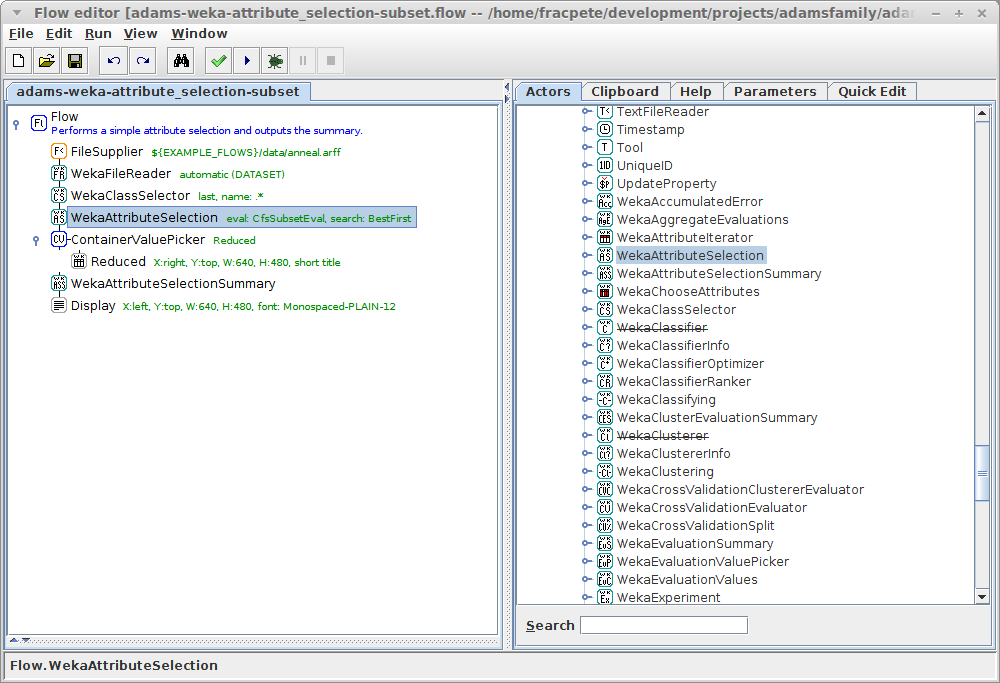
\includegraphics[width=6.0cm]{images/attribute-selection_flow.png}
  \caption{Flow for performing attribute selection (reduction).}
  \label{attribute-selection_flow}
\end{figure}

\begin{figure}[ht]
  \begin{minipage}[t]{0.5\linewidth}
    \centering
    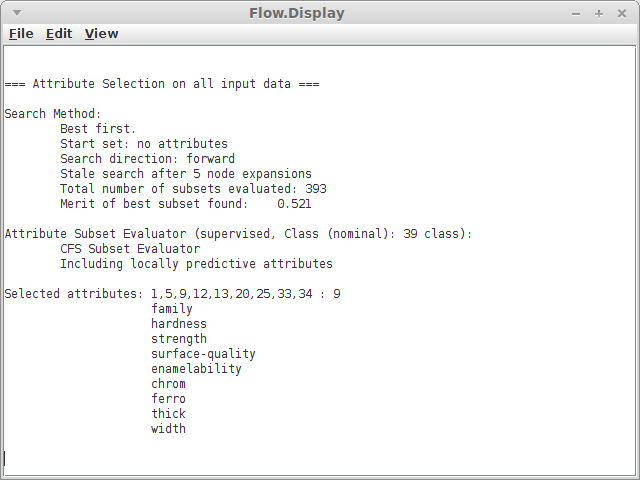
\includegraphics[width=6.0cm]{images/attribute-selection_output1.png}
    \caption{Summary of the reduction.}
    \label{attribute-selection_output1}
  \end{minipage}
  \hspace{0.5cm}
  \begin{minipage}[t]{0.5\linewidth}
    \centering
    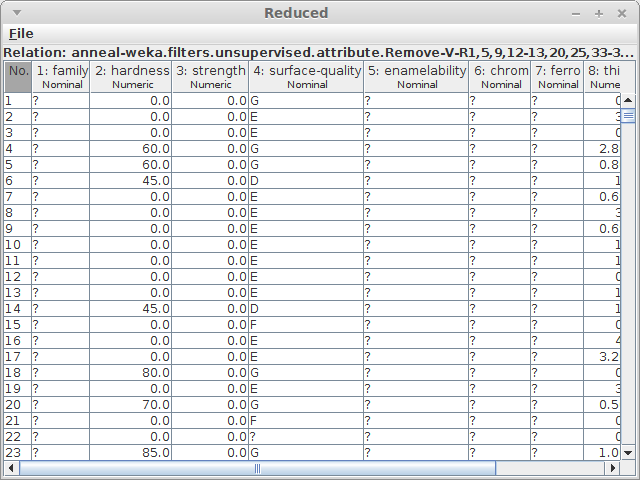
\includegraphics[width=5.5cm]{images/attribute-selection_output2.png}
    \caption{The reduced dataset.}
    \label{attribute-selection_output2}
  \end{minipage}
\end{figure}

The \textit{WekaAttributeSelection} transformer outputs a container which can 
contain the following elements:
\begin{tight_itemize}
	\item \textit{Train} -- the training set.
	\item \textit{Reduced} -- the reduced dataset.
	\item \textit{Transformed} -- the transformed dataset, in case of evaluators that 
	implement \textit{AttributeTransformer}, like principal components.
	\item \textit{Evaluation} -- the generated attribute selection evaluation.
	\item \textit{Statistics} -- a spreadsheet with statistics, containing
	information whether an attribute was selected (0 or 1) or for ranking results
	the rank of the attribute.
	\item \textit{Seed} -- the seed value in case of cross-validation.
	\item \textit{Folds} -- the number of folds used in case of cross-validation.
\end{tight_itemize}
